% LTeX: language=ro-RO

\documentclass[12pt, a4paper]{article}

\usepackage[utf8]{inputenc}      
\usepackage[T1]{fontenc}
\usepackage{geometry}  
\usepackage{graphicx}    
\usepackage{titlesec}      
\usepackage{enumitem}      
\usepackage{hyperref}         
\usepackage{float}              

\geometry{
    top=2.5cm,
    bottom=2.5cm,
    left=2.5cm,
    right=2.5cm
}


\title{\textbf{Propunere Proiect de Licență} \\ \vspace{0.5cm} \Large Platforma de Robo-Advisory pentru Optimizarea Automată a Portofoliilor de Investiții}
\author{\textbf{Student:} Andrei Opran \\ \textbf{Grupa:} 342}
\date{} 

\begin{document}

\maketitle
\vspace{1cm}

% --- Sectiunea 1 ---
\section{Rezumat}
Proiectul constă în dezvoltarea unei platforme de tip \textbf{Wealth Management Automatizat}. Acest sistem funcționează pe principiul "Set \& Forget", fiind orientat către utilizatorii care preferă o strategie pasivă de investiții, bazată pe optimizare matematică și nu pe speculație manuală.

Aplicația \textbf{gestionează integral capitalul} utilizatorului, în regim simulat de "Paper Trading". Utilizatorul depune suma de bani, iar sistemul \textbf{execută automat} ordinele de vânzare și cumpărare, rebalansează periodic portofoliul și raportează performanța, fără a fi necesară intervenția acestuia.

% --- Sectiunea 2 ---
\section{Arhitectură}
Sistemul utilizează o arhitectură de tip microservicii distribuite pe două servere care comunică printr-o rețea privată securizată (VPC), fiecare componentă fiind selectată pentru a răspunde unor cerințe specifice de performanță:

\begin{enumerate}[label=\textbf{\arabic*.}]
    \item \textbf{Nodul Operațional (Golang)}
    \begin{itemize}
        \item \textbf{Rol:} Gestionează interacțiunea cu utilizatorul, API-ul de plăți și afișarea dashboard-urilor.
        \item \textbf{Justificare:} Golang a fost ales pentru modelul eficient de concurență, esențial pentru a gestiona multiple conexiuni și cereri simultan.
    \end{itemize}
    
    \item \textbf{Nodul Decizional (Python)}
    \begin{itemize}
        \item \textbf{Rol:} Rulează algoritmi de optimizare (Markowitz) și decide compoziția portofoliului.
        \item \textbf{Justificare:} Python este standardul în industria financiară pentru calcul, având librării precum Pandas și SciPy care simplifică implementarea modelelor matematice.
    \end{itemize}
    
    \item \textbf{Baza de Date (PostgreSQL)}
    \begin{itemize}
        \item \textbf{Rol:} Persistența datelor critice (balanțe, tranzacții, portofolii).
        \item \textbf{Justificare:} S-a ales o bază de date relațională pentru consistența structurii datelor și proprietățile \textbf{ACID}. Într-o aplicație financiară, consistența tranzacțiilor este prioritară față de flexibilitatea unei baze NoSQL.
    \end{itemize}
\end{enumerate}

% --- Sectiunea 3 ---
\section{Funcționalități}

\begin{itemize}
    \item \textbf{Execuție Automată:} Robo-Advisor-ul convertește automat soldul utilizatorului în instrumente financiare (acțiuni, obligațiuni) conform calculelor interne.
    
    \item \textbf{Paper Trading și Plăți:} Integrare cu procesatoare de plăți pentru simularea completă a ciclului de alimentare card, actualizare balanță din aplicație și investiția automată.
    
    \item \textbf{Monitorizare prin Dashboard-uri:} Utilizatorul urmărește evoluția valorii totale a portofoliului și randamentul investițiilor, având vizibilitate asupra sumelor acumulate și a alocării curente a activelor.
    
    \item \textbf{Modul Opțional: Audit Log Imutabil (Blockchain)}
    \begin{itemize}
        \item \textit{Ce se auditează:} Fiecare decizie luată de Robo-Advisor și fiecare tranzacție monetară este înregistrată într-un bloc criptat.
        \item \textit{Ce se verifică:}
        \begin{itemize}
            \item \textbf{Integritatea Istoricului:} Structura de tip blockchain garantează că administratorul bazei de date nu a afectat performanța portofoliului prin modificarea acțiunilor din trecut.
            \item \textbf{Integritatea Algoritmului:} El nu ia dat cartea dar nu este deranjat. Se verifică prin checksum că nodul Python a rulat versiunea corectă a algoritmului, prevenind execuția unui cod alterat.
        \end{itemize}
    \end{itemize}
\end{itemize}

% --- Sectiunea 4 ---
\section{Tehnologii}

\begin{itemize}
    \item \textbf{Backend:} Golang (Gin Framework) + Python (Flask Microservice).
    \item \textbf{Infrastructură:} 2x Digital Ocean Droplets (Linux), comunicare prin VPC.
    \item \textbf{Bază de Date:} PostgreSQL.
    \item \textbf{Frontend:} HTML, Bootstrap, Plotly.js.
\end{itemize}

% --- Sectiunea 5 ---
\section{Diagrama Arhitectură}

\begin{figure}[H]
    \centering
    % Linia de mai jos redimensioneaza imaginea sa incapa pe inaltime (height)
    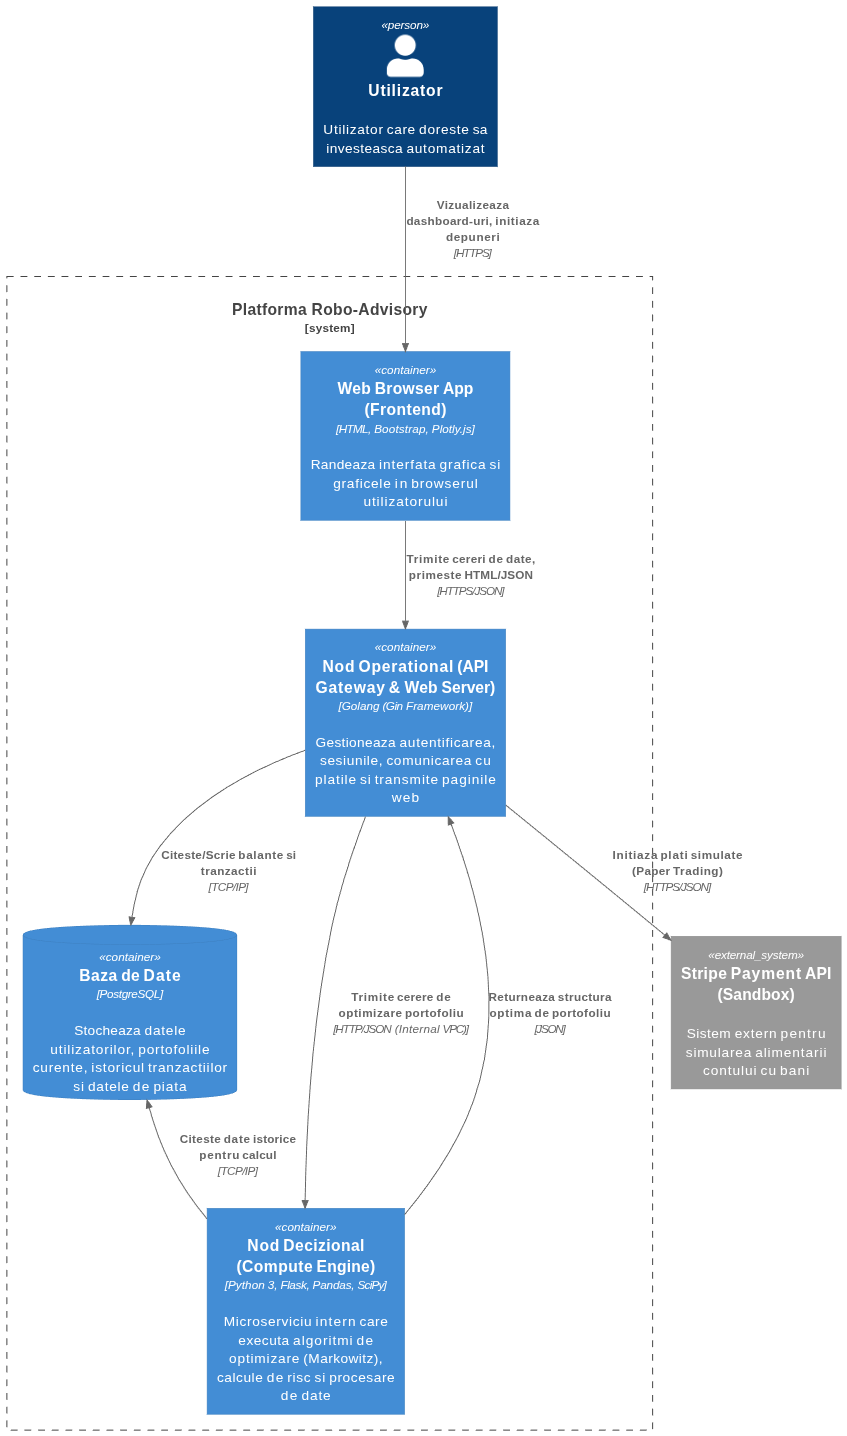
\includegraphics[height=0.85\textheight, width=\textwidth, keepaspectratio]{Propunere_Licenta_diagrama.png}
    
    \caption{Diagrama C4 Container a Platformei Robo-Advisory}
    \label{fig:arhitectura}
\end{figure}

\end{document}
